% vim: tw=80 fo=aw2tq ts=2 sw=2 et:
\documentclass{VUMIFInfBakalaurinis}
\usepackage{algorithm}
\usepackage{algorithmicx}
\usepackage{algpseudocode}
\usepackage{amsfonts}
\usepackage{amsmath}
\usepackage{bm}
\usepackage{caption}
\usepackage{color}
\usepackage{float}
\usepackage{graphicx}
\usepackage{subfig}
\usepackage{url}
\usepackage{wrapfig}

% Plotting
\usepackage{siunitx}
\usepackage{tikz}
\usepackage{pgfplots}
\pgfplotsset{compat=newest}
\usepgfplotslibrary{units}
\sisetup{round-mode=places, round-precision=2 }

% Code blocks
\usepackage{listings}
\lstset{breaklines=true}

% Title page
\university{Vilniaus universitetas}
\faculty{Matematikos ir informatikos fakultetas}
\institute{Informatikos institutas}
\department{Informatikos katedra}
\papertype{Baigiamasis bakalauro darbas}
\title{Naujausių automatizuoto slaptažodžių parinkimo metodų palyginimas}
\titleineng{Comparison of the latest automated password guessing techniques}
\status{4 kurso 1 grupės studentas}
\author{Gediminas Valys}
\supervisor{prof. dr. Igoris Belovas}
\reviewer{doc. dr. Vardauskas Pavardauskas}
\date{Vilnius \\ 2022}

\setmainfont{Palemonas}
\bibliography{bibliografija} 

\begin{document}
\maketitle

\tableofcontents

\sectionnonum{Sąvokų apibrėžimai}
Sutartinių ženklų, simbolių, vienetų ir terminų sutrumpinimų sąrašas (jeigu
ženklų, simbolių, vienetų ir terminų bendras skaičius didesnis nei 10 ir
kiekvienas iš jų tekste kartojasi daugiau nei 3 kartus).

\section{Santrauka}
Santrauka lietuviškai.

\section{Summary}
Summary in English.

\section{Įvadas}
% Autentifikacija slaptažodžiu
Vartotojo autentikacija slaptažodžiu yra vienas iš pagrindinių kibernetinio 
saugumo metodų.
% Kodėl yra poreikis slaptažodį nustatyti
Baudžiamųjų bylų tyrimuose, siekiant nustatyti kaltę, skaitmeninės informacijos 
specialistams užduodamos užduotys nuskaityti kaltinamojo kompiuterių, mobiliųjų 
įrenginių informaciją ir atlikti informacijos analizę, atsakyti į užduotyje 
pateiktus klausimus -- jei įrenginys apsaugotas skaitmeninės informacijos 
šifravimo priemonėmis, taip pat svarbu nustatyti 
prisijungimo/apsaugos/iššifravimo slaptažodį -- kitaip informacijos analizės 
atlikti nėra galimybės.
% Plačiau apie probleminę sritį
Tokiose atvejuose, kai reika iššifruoti skaitmeninę informacijos laikmeną arba 
prisijungti prie vartotojo internetinės paskyros nežinant apsaugos slaptažodį, 
naudojami slaptažodžių parinkimo metodai nustatyti apsaugos/prisijungimo 
slaptažodį -- atspėjimas brutalios jėgos būdu, naudojant įvairias nutekintas 
slaptažodžių duomenų bazes. Aukščiau minėti metodai yra ribotų galimybių -- 
brutalios jėgos būdu ilgesnius nei 6 simbolių ilgio slaptažodžius nustatyti 
praktiškai neįmanoma dėl eksponentiškai išaugusio sudėtingumo ir duomenų kiekių, 
o slaptažodžių sąrašuose tikimybė, kad yra ieškomas slaptažodis, maža.
% Tikslas - palyginti du naujausius automatizuoto slaptažodžio parinkimo 
% metodus, kurie gali ir sudėtingesnius slaptažodžius lengvai parinkti
Naujausi automatizuoto slaptažodžių parinkimo metodai, pagrįsti mašininio 
mokymosi ir statistiniais metodais, turi potencialo parinkti ir ilgesnius, nei 6 
simbolių ilgio, slaptažodžius, kurių esamuose slaptažodžių sąrašuose nėra -- šie 
metodai galėtų žymiai palengvinti ir supaprastinti slaptažodžio parinkimo 
užduotis. Šio darbo tikslas yra palyginti tokius metodus, įvertinant jų 
efektyvumą, privalumus ir trūkumus.
% Kaip aš tai atliksiu - įvardinti uždavinius, tyrimo metodologija
Iškelto tikslo pasiekimui šiame darbe bus atliekami eksperimentai su aukščiau 
minėtais slaptažodžių parinkimo metodais, kuriose siekiama parinkti kuo didesnį 
kiekį iš anksto nežinomų slaptažodžių nutekintuose slaptažodžių duomenų bazėse. 
Apmokius slaptažodžių parinkimo modelį su pasirinktomis atvirai prieinamomis 
nutekintomis slaptažodžių duomenų bazėmis bus fiksuojamas parinktų slaptažodžių, 
persidengiančių su nežinomų (ieškomų) slaptažodžių aibe, kiekis. Išbandžius 
skirtingus modelio apmokymo slaptažodžių duomenų bazes, užfiksavus ir įvertinus 
pasiektus rezultatus, vedamos išvados.

\section{Literatūros apžvalga}
\subsection{Pagrindinės idėjos}
Šioje dalyje siekiama aptarti pagrindines mintis, idėjas, kurios suteikia 
konteksto probleminei sričiai ir kuriomis vadovaujantis veikia slaptažodžio
parinkimo metodai. Kiekvienas nagrinėjamas automatizuotas slaptažodžio parinkimo 
metodas yra pagrįstas bendresnių mokslinių, technologinių pažengimų, ir yra 
konkretus jų pritaikymas slaptažodžio parinkimo problemos sprendimui, dėl to 
metodo veikimo principo apžvalgai yra reikalingos žemiau minimos pagrindinės 
mintys.

\subsubsection{Slaptažodžių parinkimo procesas} \label{sec:cracking}
Slaptažodžių parinkimas šnekamojoje kalboje taip pat vadinamas 
\textquote{slaptažodžių laužymu} -- procesas, kai turimą nežinomo slaptažodžio 
kontrolinę sumą yra bandoma atspėti parenkant tikrąjį, maišos funkcijos 
neapdorotą slaptažodį. Turint slaptažodį, kurį norima patikrinti, slaptažodis 
yra apdorojimas kriptografine maišos funkcija ir palyginama išvesta kontrolinė 
suma su turima kontroline suma -- jei kontrolinės sumos sutampa, slaptažodis 
buvo atspėtas/parinktas (\textquote{nulaužtas}).

\subsubsection{Maišos funkcija ir kontrolinė suma} \label{sec:hashing}
Kaip minėta \ref{sec:cracking} skyriuje, slaptažodžio parinkime paprastai turime 
kokio nors slaptažodžio kontrolinę sumą, sukurtą kriptografinės maišos 
funkcijos, kurios tikrąją vertę nežinome, bet galime atspėti.

Slaptažodžių parinkimui bei saugojimui yra taikomos kriptografinėmis maišos 
funkcijos (angl. \textquote{Hash Function}) dėl jų išvesties savybių. Maišos 
funkcija yra kriptografijoje naudojamas skaičiavimas (algoritmas), kuris iš tam 
tikros įvesties grąžina unikalę išvestį,
vadinamą kontroline suma (angl. \textquote{Hash}). Kontrolinė suma dalinai arba 
pilnai pasikeičia atspindint menkiausią pasikeitimą įvesties duomenyse, pvz. 
maišos funkcija \textquote{MD5} (angl. \textquote{Message Digest Algorithm 5}) 
įvestiems duomenims \textquote{duomenys} grąžina išvestį 
\textquote{df4111da0615399abad70223d1d74b9b}; pakeitus įvesties duomenų vieną 
simbolį -- įvesties duomenys dabar yra \textquote{duomenis} -- atitinkama 
\textquote{MD5} maišos funkcijos kontrolinė suma bus 
\textquote{a9d5bc509e33c1d98dca1ba876c9045b}.

Iš kontrolinės sumos įvesties duomenų atkurti paprastai neįmanoma, tačiau tarp 
skirtingų įvesties duomenų gali būti ir kolizijų -- (dalinai) sutampančių 
kontrolinių sumų, pagal kurias galima (dalinai) atspėti pradinius duomenis. 
Siekiant išvengti kolizijų, rekomenduojama naudoti stiprias kriptografines 
maišos funkcijas, kurių kolizijų tikimybės yra labai mažos, praktiškai 
neįmanomos. Kaip pavyzdį paėmus \textquote{SHA-256} kriptografinę maišos 
funkciją (angl. \textquote{Secure Hash Algorithm 256 Bit}), kurios kontrolinė 
suma yra 64 simbolių (32 baitų, 256 bitų) ilgio, sudaryta iš skaitmenų ir 
lotyniškos abėcėlės raidžių, tikimybė, kad kontrolinė suma nepasikeistų net su 
mažiausiu pasikeitimu pradiniuose duomenyse (pvz. pakeitus vieną bitą) yra 
$\frac{1}{2^{256}}$ -- beveik lygi nuliui. Palyginus su anksčiau minėtu 
\textquote{MD5} kriptografinės maišos funkcijos algoritmu, kurio kontrolinės 
sumos yra 32 simbolių (16 baitų, 128 bitų) ilgio, tikimybė, kad bus vienoda 
kontrolinė suma -- $\frac{1}{2^{128}}$. Praktikoje jau buvo rastos kolizijos su 
\textquote{MD5} algoritmu, taikant įvairias atakas ir metodus nustatyti 
kolizijas trumpiau nei per sekundę \cite{BreakMD5,MD5Attacks}.

Maišos funkcijos yra naudojamos suskaičiuoti slaptažodžių kontrolines sumas -- 
dažnai prie slaptažodžių pridedama papildoma informacija, kuri gali būti saugoma 
duomenų bazėse arba šifruotų laikmenų antraštėse. Prieš skaičiuojant 
slaptažodžio kontrolinę sumą, gera praktika yra prie slaptažodžio pridėti 
papildomą informaciją, kaip pvz. vadinamoji \textquote{druska} (angl. 
\textquote{salt}), skirta apsunkinti tam tikras slaptažodžių parinkimo atakas 
(naudojant iš anksto suskaičiuotus slaptažodžių kontrolinių sumų sąrašus, angl. 
\textquote{Rainbow Tables}). \textquote{Druska} dažnai būna atsitiktiniu būdu
parinkta simbolių, raidžių ir skaičių seka, kuri yra saugoma kartu su galutine 
slaptažodžio ir \textquote{druskos} kontroline suma. Kai vartotojas prisijungia 
prie internetinės svetainės arba įveda kompiuterio skaitmeninės laikmenos 
iššifravimo slaptažodį, įvestas slaptažodis yra sujungiamas su 
\textquote{druska} ir palyginamas su turima kontroline suma. Tokio pavidalo 
saugomus slaptažodžius yra sudėtingiau parinkti, kadangi \textquote{druskos} 
reikšmės paprastai gali siekti net iki 32 simbolių ilgio. Šiame darbe 
nagrinėjami slaptažodžio parinkimo metodai neįvertina \textquote{druskos}.

\subsubsection{Mašininis mokymasis}
Mašininis mokymasis, tame tarpe dirbtinis intelektas ir neuroniniai tinklai, 
paprastai naudojami spręsti duomenų analizės, prognozavimo, klasifikavimo ar 
naujų duomenų sintetinio generavimo problemas. Konkretus pritaikymas šiai 
technologijai yra didiesiems duomenims (angl. \textquote{Big Data}) -- masinis 
kiekis duomenų (nuo kelių šimtų megabaitų iki kelių šimtų gigabaitų ar daugiau) 
gali būti naudojami prognozuoti rinkos tendencijas, žmonių elgesį, transformuoti 
ir generuoti kitus duomenis apmokius kompiuterinį modelį įžvelgti paprastai 
nematomus požymius duomenyse. Mašininiui mokymuisi yra reikalingi dideli duomenų 
kiekiai siekiant sumažinti galimų klaidų skaičių, pagrindinis būdas tai atlikti 
yra apmokyti mašininio mokymosi modelį su visomis (kuo daugiau) galimomis 
įvesties reikšmėmis. Mašininio mokymosi modelis -- parametrų ir duomenų 
rinkinys, kurie yra nustatomi, koreguojami ir/ar surenkami modelio apmokymo 
procese, kuris yra taikomas spręsti aukščiau minėtas problemas.

Internete paplitusios nutekintos slaptažodžių duomenų bazės yra laisvai 
prieinami, dideli (nuo kelių šimtų megabaitų iki kelių šimtų gigabaitų) duomenų 
rinkiniai, tinkami mašininio mokymosi metodų pritaikymui slaptažodžio 
parinkimui.

Išskiriami du pagrindiniai mašininio mokymosi proceso tipai:
\begin{itemize}
  \item su mokytoju (angl. \textquote{Supervised Learning}) -- mašininio 
    mokymosi algoritmui yra pateikiami iš anksto suklasifikuoti, apdoroti 
    duomenys, kuriuose algoritmas turi identifikuoti tokius reikšmingus 
    požymius, kad modelio priimami sprendimai sutaptų su mokytojo nustatytais 
    sprendimais.
    Algoritmo pradiniai duomenyse kiekvienai reikšmei yra priskirta tam tikra 
    žymė (asociacija), ir algoritmas duomenyse esamus požymius (pvz. forma, 
    struktūra, pasiskirstymą, spalvą ir pan.) susieja su priskirta žyme. 
    Mokymasis su mokytoju toliau gali būti skirstomi į du tipus:
    \begin{itemize}
      \item klasifikacija -- priskirti duomenis prie tam tikros klasės, grupės;
      \item regresija -- prognozuoti duomenis, priklausančius nuo kitų duomenų.
    \end{itemize}
  \item be mokytojo (angl. \textquote{Unsupervised Learning}) -- mašininio 
    mokymosi algoritmui yra pateikiami \textquote{žali} duomenys, t.y. ne 
    klasifikuoti ar kitaip apdoroti, ir modelis turi pats identifikuoti, 
    išskirti duomenyse reikšmingus požymius, ryšius. Mokymasis be mokytojo 
    toliau gali būti skaidomas į du tipus:
    \begin{itemize}
      \item grupavimas -- reikšmių padalijimas į grupes, kurios turi panašius 
        požymius;
      \item asociacija -- taisyklėmis pagrįstas mokymasis, kuriame nustatomi 
        tarpusavio ryšiai tarp reikšmių.
    \end{itemize}
\end{itemize}

\subsection{Brutalios jėgos metodas slaptažodžio parinkimui} 
\label{sec:bruteforce}
Vienas iš tradicinių, paprasčiausių būdų automatizuoto slaptažodžio parinkimui 
yra brutalia jėga (angl. \textquote{Brute Force}), t.y. sugeneruoti visas 
įmanomas slaptažodžių reikšmes nustatyto ilgio (ilgių intervale) su pasirinkta 
simbolių (raidžių, skaitmenų ir specialių simbolių) aibe ir atlikti slaptažodžių 
parinkimą pagal \ref{sec:cracking} skyriuje aprašytą metodiką.

Pavyzdžiui, jei vartotojas turėtų iki 6 simbolių ilgio slaptažodį, tai programa 
ar kompiuteris galėtų sugeneruoti visus įmanomus 1-6 simbolių ilgio 
slaptažodžius, su visomis raidžių, skaičių ir simbolių (mišinių) permutacijomis, 
ir, jeigu tinkamai parinkta simbolių aibė, galima garantuoti, kad vartotojo 
slaptažodis yra tarp sugeneruotų.

Su šiuo metodu, generuojamų slaptažodžių kiekis eksponentiškai auga priklausant 
nuo slaptažodžio ilgio ir simbolių aibės, ir net 6 simbolių ilgių slaptažodžių 
sąraše, jei naudojamą simbolių aibę sudaro 95 simboliai, iš viso yra $95^6$ 
(arba $735091890625$) galimi slaptažodžiai, žr. \ref{tab:bruteforce} pav.

\begin{table}[hb]
  \centering
  \begin{tabular}{|c|c|}
    \hline \textbf{Ilgis} & \textbf{Kiekis} \\
    \hline 1 & 95 \\
    \hline 2 & 9025 \\
    \hline 3 & 857375 \\
    \hline 4 & 81450625 \\
    \hline 5 & 7737809375 \\
    \hline 6 & 735091890625 \\
    \hline
  \end{tabular}
  \caption{
    Slaptažodžių kiekių augimas priklausant nuo slaptažodžio ilgio, 95 simbolių 
    aibėje (\textquote{ASCII} koduotėje).
  }
  \label{tab:bruteforce}
\end{table}

Atitinkamai paskaičiavus tokių duomenų kiekių, kaip pavaizduotų 
\ref{tab:bruteforce} lent., talpą skaitmeninėje atmintyje (laikmenoje) pvz. 
visiems 6 simbolių ilgio slaptažodžiams, slaptažodžiai užimtų apie $3859$ 
gigabaitų (su prielaida, kad simboliai yra \textquote{ASCII} koduotės ir 
kiekvienas simbolis užima po 8 bitus).

\textquote{Python} programine kalba parašytu scenarijumi, pateiktame 
\ref{fig:permutacijos} pav., sugeneravau visas 5 simbolių permutacijas 
(\textquote{ASCII} koduotėje) per $88.4$ minutes, kurios sudaro 6952862280 
eilutes (slaptažodžius) ir užima $39$ gigabaitų talpos skaitmeninėje laikmenoje.

\begin{figure}
  \begin{center}
    \lstinputlisting[
      language=Python,
      numbers=left
    ]{permutations.py}
    \caption{Programinis kodas sugeneruoti visas 5 simbolių kombinacijas.}
    \label{fig:permutacijos}
  \end{center}
\end{figure}

Ilgesnius slaptažodžius, nei 6 simbolių ilgio, brutalios jėgos metodu parinkti 
nebėra nei praktiška, nei realu, kadangi duomenų kiekiai išauga virš $4107$ 
gigabaitų (su prielaida, kad simboliai yra \textquote{ASCII} koduotės ir 
kiekvienas simbolis užima po 8 bitus).

\subsection{Slaptažodžių sąrašai slaptažodžio parinkimui} \label{sec:wordlists}
Internete paplitusios vartotojų slaptažodžių nutekintos duomenų bazės yra 
tinkamos slaptažodžių parinkimui. Vartotojai dažnai naudoja tuos pačius 
slaptažodžius daugeliui savo kuriamų internetinių svetainių paskyrų, tačiau 
nebūtinai visi šių internetinių svetainių kūrėjai/aptarnautojai laikosi
informacinės saugos taisyklių ir gerųjų praktikų, tokių, kaip:
\begin{enumerate}
  \item nesaugoti slaptažodžius paprastu tekstu (angl. \textquote{Plain Text}), 
        o apdoroti slaptažodžius stipriomis kriptografinėmis maišos funkcijomis;
  \item su \textquote{druska} apsaugoti slaptažodžius nuo dažniausiai naudojamų 
        atakų, kaip pateikta \ref{sec:hashing} skyriuje.
\end{enumerate}

Kai veikėjas (asmuo, programa) įsiveržia į tokias internetines svetaines ir 
nutekina prisiregistravusių vartotojų asmeninius duomenis, tame tarpe ir 
prisijungimo slaptažodžius, jie būna parduodami internete arba patalpinami 
nemokamai laisvai prieinamuose internetinėse svetainėse.
% TODO Gal įdėti pavyzdžių kokių nors populiariausių tokių wordlistų?
Naudojantis šias duomenų bazes su vartotojų prisijungimo informacija, kiekvienas 
slaptažodis yra apdorojamas maišos funkcija ir jos išvesta kontrolinė suma 
palyginama su turimomis nežinomomis slaptažodžių kontrolinių sumomis.

\subsection{Slaptažodžių kontrolinių sumų sąrašai slaptažodžio parinkimui} 
\label{sec:rainbowtables}
Slaptažodžių apdorojimui į kontrolines sumas, naudojant kriptografines maišos 
funkcijas, tokiais dideliais kiekiais, kaip nutekintų slaptažodžių duomenų 
bazių, reikalingi dideli kompiuteriniai ištekliai. Siekiant minimizuoti laiką, 
skirtą slaptažodžio parinkimui, nutekintos slaptažodžių duomenų bazės (ar jų 
mišinio) slaptažodžiai yra iš anksto apdorojami kriptografinės maišos funkcijos 
(toks metodas vadinamas angl. \textquote{Rainbow Tables}). Tokiu būdu, 
slaptažodžio užpuolikui, siekiančiam nustatyti tikrąją slaptažodžio reikšmę, 
reikia tik palyginti kontrolines sumas ir surasti, jei tokia yra, sutampančią. 
Kaip minėta \ref{sec:hashing} skyriuje, tokio tipo ataka netinkama 
slaptažodžiams, kurie yra apsaugoti su \textquote{druska}, kadangi kontrolinės 
sumos skirtųsi net ir jeigu tikra slaptažodžio reikšmė sutampa.

Paminėtina, kad naudojantis tokiais sugeneruotais sąrašais, kaip pateikta 
\ref{sec:bruteforce}, \ref{sec:wordlists} ir \ref{sec:rainbowtables} skyriuose, 
vartotojas galėtų paskirstyti skaičiavimus (slaptažodžio parinkimą) kelioms 
procesoriaus gijoms, vaizdo plokštėms ar kompiuteriams slaptažodžių sąrašą 
padalinant į dalis, siekiant pagreitinti slaptažodžio parinkimą.

% \subsection{Slaptažodžių transformavimas naudojant taisykles}
% Atvirojo kodo programinė įranga \textquote{hashcat}\footnotemark, skirta 
% slaptažodžių atstatymui - nustato tikrąjį slaptažodį taikant brutalios jėgos ir 
% kt. metodus turimo slaptažodžio kontrolinei sumai -- palaiko teksto eilučių 
% (slaptažodžių) transformavimą taisyklėmis. Taisyklės yra tekstiniai failai, 
% kuriose yra pateiktos instrukcijos kaip transformuoti žodyno ar kitus žodžius. 
% Pavyzdžiui, kaip bus matyti \ref{tab:rockyou10} lentelėje, dauguma žmonių 
% parenka paprastus, raidinius ar skaitmenų slaptažodžius. Mažesnė dalis žmonių 
% pakeičia raides skaitmenimis, simboliais, didžiąsias raides į mažąsias ar 
% atvirkščiai ir pan. Atsižvelgiant į tokias transformacijas, yra 6561 skirtingos 
% slaptažodžio \textquote{password} versijos, kurias kompiuteris gali įveikti 
% 
% \footnotetext{
%   Programinės įrangos internetinė svetainė: \url{https://hashcat.net/hashcat/}.
% }

\subsection{Ankstesni darbai}
Automatizuoto slaptažodžio parinkimo metodų srityje yra atlikti moksliniai 
tyrimai, nagrinėjantys galimybes pritaikyti ir integruoti mašininį mokymąsi bei 
kitus metodus, kad slaptažodžio parinkimo procesas sudėtingesniems, nei 1-6 
simbolių ilgio slaptažodžiams, vyktų lengviau (greičiau). Šie metodai 
automatizuotu būdu generuoja taisykles (požymius) iš pradinių duomenų (paprastai 
naudojamos nutekintos slaptažodžių duomenų bazės), ir pagal sugeneruotas 
taisykles (požymius) -- naujus slaptažodžius. Žemiau yra paminėti keli tokie 
metodai:
\begin{enumerate}
  \item \textquote{PassGAN} -- paremtas mašininio mokymosi generatyviniais 
    konkurenciniais tinklais \cite{PassGAN};
  \item \textquote{PCFG} -- paremtas tikimybine bekontekste gramatika 
    \cite{PCFG1,PCFG2};
  \item \textquote{GenPASS} -- pagrįstas mašininio mokymosi pasikartojančiais 
    neuroniniais tinklais ir tikimybiniais gramatikos taisyklių rinkiniais 
    \cite{GenPASS};
  \item \textquote{TG-SPSR} -- slaptažodžių parinkimo strategija, pagrįsta 
    tikimybiniais gramatikos taisyklių rinkiniais ir Markovo grandinių modeliais 
    \cite{TG-SPSR}.
\end{enumerate}

Peržiūrėjus aukščiau minėtus mokslinius darbus nuspręsta palyginti ir nagrinėti 
\textquote{PassGAN} ir \textquote{PCFG} metodus, kadangi \textquote{PassGAN} 
metodas naudoja tik mašininį mokymasį, \textquote{PCFG} metodas -- tik 
statistinę analizę. Kiti metodai integruoja mašininį mokymasį, statistinę 
analizę.
% Ne tik pasakyti ką atliko kiti autoriai, bet palyginti jų darbus, pateikti tų 
% darbų pliusus ir minusus

% Kaip veikia šitas algoritmas, pateikti pavyzdžių (įdėti transformacijų medį)

% Kokie šio algoritmo pagrindiniai požymiai, pastebėti trūkumai ir minusai
% TODO parasyti apie kitus algoritmus
% idet kas yra masininis mokymasis ir pan, viska aprasyt kad belekas suprastu,
% isivaizduot kad bet kokios srities zmogus skaito, ir aprasyt taip, kad 
% suprastu

\subsubsection{\textquote{PassGAN} metodas}
Šioje dalyje atliksiu apžvalgą generatyvinių konkurencinių tinklų (angl. 
\textquote{Generative Adversarial Networks}), pagal kuriuos yra pagrįstas 
\textquote{PassGAN} metodas, bei pateiksiu jų esminius automatizuoto 
slaptažodžių parinkimo pritaikymo bruožus.

% Kas yra GANai
% Pritaikymas slaptažodžių parinkimo srityje
% Kaip algoritmas veikia
\subsubsubsection{Apie generatyvinius konkurencinius tinklus}
Generatyviniai konkurenciniai tinklai (angl. \textquote{Generative Adversarial 
Networks}, \textquote{GAN}) yra generatyvinis modeliavimas naudojant gilaus 
mašininio mokymosi metodus. Generatyvinis modeliavimas yra mašininio mokymosi 
metodas be mokytojo, kuriame modelis yra apmokamas generuoti tokias reikšmes, 
kurios galėtų tikėtinai būti iš apmokymo duomenų rinkinio. Generatyviniame 
konkurenciniame tinkle yra dvi dalys -- generavimo modelis (angl. 
\textquote{Generator Model}), kuris yra apmokamas generuoti naujas reikšmes, ir 
diskriminatoriaus modelis (angl. \textquote{Discriminator model}), kuris 
klasifikuoja generuojamas reikšmes kaip tikras arba netikras. Generatyvinių 
konkurencinių tinklų pagrindas yra žaidimas tarp dviejų konkuruojančių 
neuroninių tinklų, kuriame minėti du modeliai konkuruoja ir varžosi -- vienas 
modelis generuoja reikšmes, kitas bando atskirti jas nuo generuotų duomenų ir 
apmokymo duomenų \cite{DL,GAN}. Generavimo modelis yra apmokamas tol, kol 
generuoja tokias įtikinamas reikšmes, kurias diskriminatoriaus modelis negali 
atskirti nuo realių (apmokymo) reikšmių, t.y. generavimo modelis apmokamas tol, 
kol neapgauna diskriminatoriaus modelio \cite{GAN}.

Pagrindinis skirtumas tarp diskriminuojančio ir generatyvinio modeliavimo yra 
tai, diskriminacinis modelis klasifikuoja -- turi būti priimtas sprendimas, 
kuriai klasei priklauso tam tikra reikšmė, o generatyvinis -- generuoja arba 
sukuria naujas reikšmes pagal pradinius duomenis, kurie galėtų tikėtinai būti 
pradiniame duomenų rinkinyje. Kitaip tariant, generatyvinis modelis gali būti 
apmokytas pradinių duomenų pasiskirstymo ir gali generuoti naujas reikšmes, 
kurios galėtų tikėtinai būti priskirtos prie pradinių duomenų \cite{PRaML}.

Generavimo modeliui yra pateikiama kaip įvestis nustatyto ilgio vektorius iš 
atsitiktinai paskirstytos duomenų aibės (angl. \textquote{Gaussian 
Distribution}). Apmokymo metu tam tikriems (paprastai nematomiems) požymiams iš 
šios duomenų aibės yra priskiriama svarba, t.y. generuojamos reikšmės artėja 
prie apmokymo duomenų aibės -- generatorius sugeneruoja grupę reikšmių, kurios, 
kartu su apmokymo duomenimis, yra perduodami diskriminatoriui klasifikuoti kaip 
tikros arba netikros. Tokiu būdu kiekvieną apmokymo iteraciją diskriminatoriaus 
parametrai yra tobulinami tiksliau klasifikuoti tikras/netikras reikšmes, o 
generatorius -- kiek sugeneruotos reikšmės galėjo apgauti/įtikinti 
diskriminatorių (diskriminatoriaus reikšmės, nustatytos kaip tikros arba 
netikros, atskleidžia reikalingą informaciją apie apmokymo duomenų aibę 
generatoriui, kuris gali ją naudoti tiksliau modeliuoti apmokymo duomenų 
pasiskirstymą). Po modelio apmokymo, minėta duomenų aibė turėtų modeliuoti 
apmokymo duomenų aibę, t.y. diskriminatorius negali su didesniu nei apie 50 \% 
tikslumu (pasitikėjimu, arba angl. \textquote{Confidence}) atskirti apmokymo 
duomenų aibės reikšmes nuo generuojamų reikšmių.

\subsubsubsection{Neuroninių tinklų struktūros}
Šiame metode naudojamas generatyvinis konkurencinis tinklas su struktūra, 
paremta \cite{GAN}, kuri yra pateikta \ref{plot:passgang}, \ref{plot:passgand} 
pav., ir \textquote{ADAM} optimizatorius \cite{ADAM} siekiant minimizuoti 
apmokymo klaidą (angl. \textquote{Training Error}).




Aprašyti neuroninio tinklo struktūrą, paaiškinti straipsnyje pasirinktus 
sprendimus/priežastis, kokie parametrai ir koks optimizatorius naudojamas ir 
kodėl.

\subsubsubsection{Pritaikymas slaptažodžių parinkimui}
Generatyviniai konkurenciniai tinklai gali būti taikomi ir naujų slaptažodžių 
sintezei, taip parenkant naujus slaptažodžius. Iš apmokymo duomenų -- nutekintų 
slaptažodžių duomenų bazių -- generavimo modelis išmoksta slaptažodžių požymius 
pagal tai, ar generuojami slaptažodžiai suklasifikuoti kaip tikri ar ne tikri 
diskriminatoriaus modelio.

\subsubsubsection{Pastebėjimai}
\textquote{PassGAN} metodas parenka daugiau slaptažodžiu su didesniu kiekiu 
generuojamų slaptažodžių, t.y. kuo didesnis sugeneruotų slaptažodžių kiekis, tuo 
daugiau parenkamų slaptažodžių nežinomų slaptažodžių aibėje -- šio metodo 
moksliniame straipsnyje atliktas tyrimas parodo, kad modelis, apmokytas su 80 \% 
\textquote{RockYou} nutekintos slaptažodžių duomenų bazės rinkinio slaptažodžių 
aibe, testuojamas su 20 \% tos pačios duomenų bazės testavimo duomenų ir 
\textquote{Linknedin} duomenų aibėmis, parenka slaptažodžius kiekiais, 
apibrėžtais \ref{tab:passganoriginalrockyouresults}, 
\ref{tab:passganoriginallinkedinresults} lent., kurioje matyti, kad su kuo 
didesniu kiekiu sugeneruotų slaptažodžių, tuo didesnis yra parinktų slaptžodžių 
skaičius testavimo duomenų aibėje. Pastebėtina, kad iš $10^10$ sugeneruotų 
slaptažodžių tik $21.5282$ \% sudaro unikalios reikšmės, t.y. $78.4718$ \% visų 
slaptažodžių yra dublikatai.

\begin{table}[hb]
  \centering
  \caption{
    Slaptažodžių, sugeneruotų \textquote{PassGAN} metodu, apmokytų 80 \% 
    \textquote{RockYou} duomenų ir sutampančių su \textquote{RockYou} testavimo 
    duomenų aibe \cite{PassGAN}.
  }
  \begin{tabular}{|c|c|c|}
    \hline \textbf{Slaptažodžių kiekis} & \textbf{Unikalūs slaptažodžiai} & 
    \textbf{Sutampančių slaptažodžių kiekis} \\
    \hline $10^4$ & 9738 & $0.005$ \% \\
    \hline $10^5$ & 94400 & $0.048$ \% \\
    \hline $10^6$ & 855972 & $0.381$ \% \\
    \hline $10^7$ & 7064483 & $2.038$ \% \\
    \hline $10^8$ & 52815412 & $6.726$ \% \\
    \hline $10^9$ & 356216832 & $15.094$ \% \\
    \hline $10^{10}$ & 2152819961 & $26.036$ \% \\
    \hline
  \end{tabular}
  \label{tab:passganoriginalrockyouresults}
\end{table}

% \begin{table}[hb]
%   \centering
%   \caption{
%     Slaptažodžių, sugeneruotų \textquote{PassGAN} metodu, apmokytų 80 \% 
%     \textquote{RockYou} duomenų ir sutampančių su \textquote{Linkedin} testavimo 
%     duomenų aibe \cite{PassGAN}.
%   }
%   \begin{tabular}{|c|c|}
%     \hline \textbf{Slaptažodžių kiekis} & \textbf{Sutampančių slaptažodžių 
%     kiekis} \\
%     \hline $10^4$ & $0.005$ \% \\
%     \hline $10^5$ & $0.048$ \% \\
%     \hline $10^6$ & $0.381$ \% \\
%     \hline $10^7$ & $2.038$ \% \\
%     \hline $10^8$ & $6.726$ \% \\
%     \hline $10^9$ & $15.094$ \% \\
%     \hline $10^{10}$ & $26.036$ \% \\
%     \hline
%   \end{tabular}
%   \label{tab:passganoriginallinkedinresults}
% \end{table}

Atlikus analizę \textquote{PassGAN} metodu sugeneruotų slaptažodžių dublikatų 
kiekio, rezultatai pateikti \ref{plot:passganoriginalresults} pav.

\begin{figure}[!ht]
  \begin{center}
    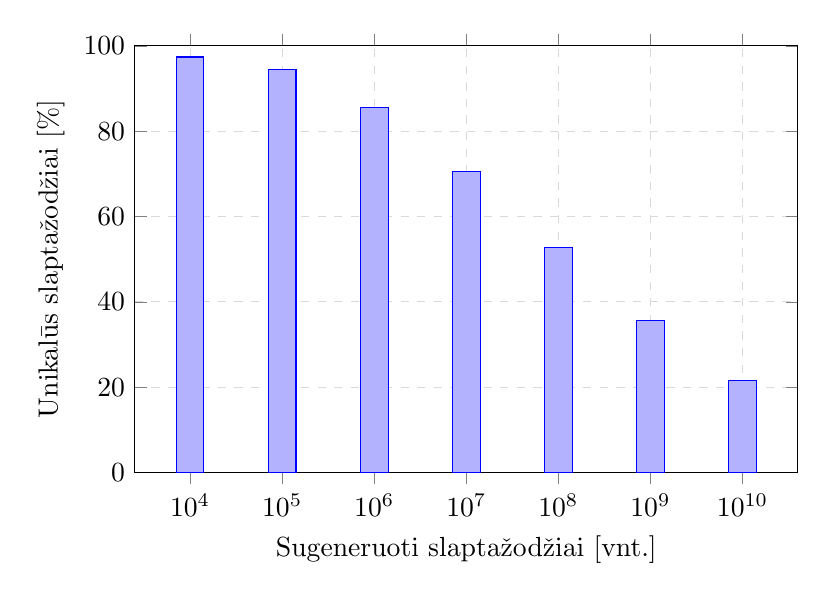
\begin{tikzpicture}
      \begin{axis}[
        ybar,
        xlabel={Sugeneruoti slaptažodžiai},
        ylabel={Unikalūs slaptažodžiai},
        x unit={vnt.},
        y unit={\%},
        ymin=0,
        ymax=100,
        xticklabels={,,$10^4$,$10^5$,$10^6$,$10^7$,$10^8$,$10^9$,$10^{10}$},
        grid=major,
        grid style={dashed,gray!30},
        width=10cm,
        height=7cm,
      ]
      \addplot coordinates {
        (1, 97.38)
        (2, 94.4)
        (3, 85.5972)
        (4, 70.64483)
        (5, 52.815412)
        (6, 35.621683)
        (7, 21.5282)
      };
      \end{axis}
    \end{tikzpicture}
  \end{center}
  \caption{
    Unikalių slaptažodžių, sugeneruotų \textquote{PassGAN} metodu, kiekis.
  }
  \label{plot:passganoriginalresults}
\end{figure}

\subsubsection{\textquote{PCFG} metodas}
\subsubsubsection{Apie tikimybinės, bekontekstes gramatikas}
\textquote{PCFG} (angl. \textquote{Probabilistic Context Free Grammar}) -- 
tikimybinis gramatikos taisyklių rinkinys, nurodantis, kaip kažkurį tai 
simbolį-reikšmę galima transformuoti į kitą simbolį. \textquote{PCFG} algoritmas 
yra pagrįstas bekontekste gramatika (angl. \textquote{Context Free Grammar}) -- 
notacija, skirtą apibrėžti tam tikros formalios kalbos sintaksę, pvz. 
programinio kodo šaltinių failų analizei ir apdorojimui į simbolių grupių 
leksinį medį (kaip simbolių grupės yra susijusios su viena kita, ką jos 
reiškia). Tikimybinė bekontekstė gramatika (angl. \textquote{Probabilistic 
Context Free Grammar}) yra bekontekstė gramatika, kurioje kiekvienai simbolių 
grupei yra priskirta tikimybė. Tikimybinė bekontekstė gramatika yra kilusi iš 
kompiuterinės lingvistikos srities, skirta analizuoti ir modeliuoti natūralią 
kalbą -- simbolių grupių (pasikartojimo) tikimybės gali būti naudojamos kaip 
parametrai mašininio mokymosi modelyje, tačiau tikimybių reikšmės ypač priklauso 
nuo duomenų (kiekio, įvairovės), iš kurių jos yra išvestos.

\subsubsubsection{Pritaikymas slaptažodžių parinkimui}
Tikimybinės bekontekstės gramatikos metodą galima pritaikyti ir slaptažodžių 
gramatikos (formalios kalbos notacijos) nustatymui, ir, pagal šią gramatiką, 
parinkti naujus slaptažodžius. Naujų slaptažodžių parinkimui yra saugomos 
simbolių grupių reikšmės -- slaptažodžiai yra dalinami ir sugrupuojami į 
sujungtas skaitmenų, raidžių ir specialiųjų simbolių grupes, kurios yra 
įstatomos į slaptažodžio gramatiką parenkant naujus slaptažodžius.

\subsubsubsection{Algoritmo apžvalga} \label{sec:pcfgalg}
Slaptažodžių parinkimo strategijoje, \textquote{PCFG} algoritmas kiekvienam 
slaptažodžiui iš apmokymo duomenų rinkinio pirmiausia išveda gramatiką, t.y. 
simbolių grupės yra sugrupuojamos pagal tipą: skaitmenys, raidės, specialūs 
simboliai ir kartu užfiksuojami su konkrečių simbolių sekų bei pačios gramatikos 
pasikartojimų skaičiumi medžio pagrindo duomenų struktūroje (paprastai binarinis 
medis, angl. \textquote{Binary Tree}). Kai visi slaptažodžiai yra apdoroti į jų 
atitinkamas gramatikas, paskaičiuojami gramatikų ir simbolių grupių 
pasikartojimo dažniai -- kiek kartų gramatika ir ją sudarančios simbolių grupių 
reikšmės pasikartoja visoje apmokymo duomenų aibėje. Minėti dažniai yra 
naudojami parenkant naujus slaptažodžius -- pirmiausia parenkami slaptažodžiai, 
kurių gramatika ir gramatikoje esančių simbolių grupių dažniai yra didžiausi, 
tokiu būdu slaptažodžiai su aukščiausia tikimybe yra parenkami pirmi. Kitaip 
tariant, slaptažodžiai, kurių forma, struktūra ir skaitmenų, raidžių, specialių 
simbolių junginių grupės pasikartoja daugiausiai, sudaro šio metodo pirmąsias 
išvestis.
Viena gramatika \textquote{PCFG} algoritme gali būti panaudota kelis kartus 
parenkant slaptažodžius. \textquote{PCFG} algoritme yra išskiriami du tipai 
slaptažodžių -- preliminarūs (angl. \textquote{Pre-terminal}) ir galutiniai 
(angl. \textquote{Terminal}). Kiekvienas preliminarus slaptažodis yra parenkamas 
atsižvelgiant į jo ašies reikšmę, t.y. simbolių grupės, kuri buvo 
pakeista/transformuota parenkant šį slaptažodį, indeksas (pirminė ašies reikšmė 
parenkant pirmuosius preliminarius slaptažodžius yra lygi nuliui). Galutinių 
slaptažodžių parinkimo ir preliminarių slaptažodžių transformavimo taisyklės yra 
tokios:
\begin{enumerate}
  \item preliminariame slaptažodyje simbolių grupė gali būti keičiama tik jei 
    preliminaraus slaptažodžio ašies vertė yra mažesnė už grupės indeksą 
    slaptažodžio gramatikoje;
  \item preliminaraus slaptažodžio nauja ašis yra slaptažodyje pakeistos 
    simbolių grupės indeksas, skaičiuojant nuo 0;
  \item iš preliminaraus slaptažodžio yra parenkamas galutinis slaptažodis kai 
    yra pakeičiama viena ir tik viena simbolių grupė.
\end{enumerate}

Vadovaujantis aukščiau minėtomis taisyklėmis yra parenkami nauji galutiniai ir 
preliminarūs slaptažodžiai su transformuotomis simbolių grupėmis. Galutinis 
slaptažodis yra grąžinamas algoritmo, kai nebėra daugiau transformacijų, kurios 
galėtų būti su juo atliktos, o nauji preliminarūs slaptažodžiai, kuriems jau 
buvo atliktos transformacijos, yra grąžinami į algoritmo sąrašą tolesnėms 
transformacijoms.

Imant konkretų pavyzdį, tarkime metodas apdorojo slaptažodžių sąrašą ir sudarė 
sąrašą gramatikų ir raidžių, specialių simbolių, skaitmenų, bei jų pasikartojimo 
tikimybėmis. Šiam pavyzdžiui minėtas raidžių, specialių simbolių ir skaitmenų 
sąrašas pateiktas \ref{tab:pcfgvalues} lent.
\begin{table}[hb]
  \centering
  \caption{
    Slaptažodžių kiekių augimas priklausant nuo slaptažodžio ilgio, 95 simbolių 
    aibėje (\textquote{ASCII} koduotėje).
  }
  \begin{tabular}{|c|c|c|}
    \hline \textbf{Gramatikos grupė} & \textbf{Reikšmė} & \textbf{Tikimybė} \\
    \hline A4 & pass & 0.8 \\
    \hline A3 & App & 0.75 \\
    \hline A3 & dSA & 0.74 \\
    \hline A3 & aOS & 0.72 \\
    \hline A2 & qw & 0.68 \\
    \hline S3 & \^\&* & 0.64 \\
    \hline S2 & !* & 0.55 \\
    \hline S2 & @@ & 0.48 \\
    \hline S2 & .( & 0.45 \\
    \hline S1 & \% & 0.36 \\
    \hline S1 & \$ & 0.3 \\
    \hline D3 & 123 & 0.25 \\
    \hline D2 & 33 & 0.25 \\
    \hline D2 & 47 & 0.24 \\
    \hline D2 & 29 & 0.12 \\
    \hline
  \end{tabular}
  \label{tab:pcfgvalues}
\end{table}
Tarkime, kad pirmoji (aukščiausios tikimybės) slaptažodžio gramatika yra 
\textquote{A3S2D2}, kurią galima skaityti taip -- slaptažodį sudaro trys raidės, 
du specialiūs simboliai ir du skaitmenys. Ši gramatika buvo sugeneruota metodui 
išanalizavus slaptažodžius, kurių daugumą sudarė aukščiau minėta struktūra ir 
forma, neatsižvelgiant į kokios raidės, specialūs simboliai ir skaitmenys minėtą 
gramatiką sudarė. Inicijavus šią gramatiką išsaugotomis (sukauptomis) raidžių, 
specialių simbolių ir skaitmenų simbolių grupėmis (reiškiniais), kurie 
daugiausia pasikartoja tarp išanalizuotų slaptažodžių, galime gauti slaptažodį 
\textquote{App!*33}, kurio pradinė ašies reikšmė yra lygi nuliui. Parenkant 
pradines reikšmes pirminiams slaptažodžiams, pirmenybė skiriama reikšmėms su 
aukščiausia tikimybe (t.y. dažniausiai pasikartojo išanalizuotuose 
slaptažodžiuose). Atsižvelgiant į šio pradinio slaptažodžio ašies reikšmę (kuri 
yra lygi nuliui), galima atlikti tris transformacijas -- pakeisti grupes 
\textquote{A3}, \textquote{S2} ir \textquote{D2}, t.y. pakeisti kiekvieną 
simbolių grupę arba reiškinį vieną kartą, sugeneruojant 3 naujas šio 
slaptažodžio variacijas, po vieną kiekvienai transformacijai. Pakeitus grupę 
\textquote{A3}, ašies reikšmę -- nulį -- pakeičiame grupės indeksu -- nuliu 
(kadangi indeksą skaičiuojame nuo nulio), ir tai atlikus kitoms grupėms 
atitinkamai gauname jų ašies indeksus 1 ir 2. Taikant skyriuje \ref{sec:pcfgalg} 
pateiktas slaptažodžių transformavimo taisykles, atsižvelgiant į naujai 
sugeneruotų (transformuotų) 3 slaptažodžių ašies indeksus -- 0, 1 ir 2 -- galima 
toliau atlikti tokias transformacijas, kai šie minėti trys transformuoti 
slaptažodžiai bus išvesti:
\begin{itemize}
  \item iš pirmo transformuoto slaptažodžio, kurio ašies indeksas yra lygus 
    nuliui, išvesti 3 naujus transformuotus slaptažodžius, pakeitus 1-3 grupes;
  \item iš antro transformuoto slaptažodžio, kurio ašies indeksas yra lygus 
    vienam, išvesti 2 naujus transformuotus slaptažodžius, pakeitus 2-3 grupes;
  \item iš trečio transformuoto slaptažodžio, kurio ašies indeksas yra lygus 
    dviem, išvesti 1 naują transformuotą slaptažodį, pakeitus 3 grupę.
\end{itemize}

Grupių (reiškinių) pakeitimai yra atliekami tol, kol transformacijų ašies 
reikšmė nepasiekia paskutinės grupės, arba nepasibaigia simbolių grupės 
(reiškiniai), su kuriais būtų galima atlikti šiuos pakeitimus, žr. 
\ref{plot:pcfgtransforms} pav.

\begin{figure}
  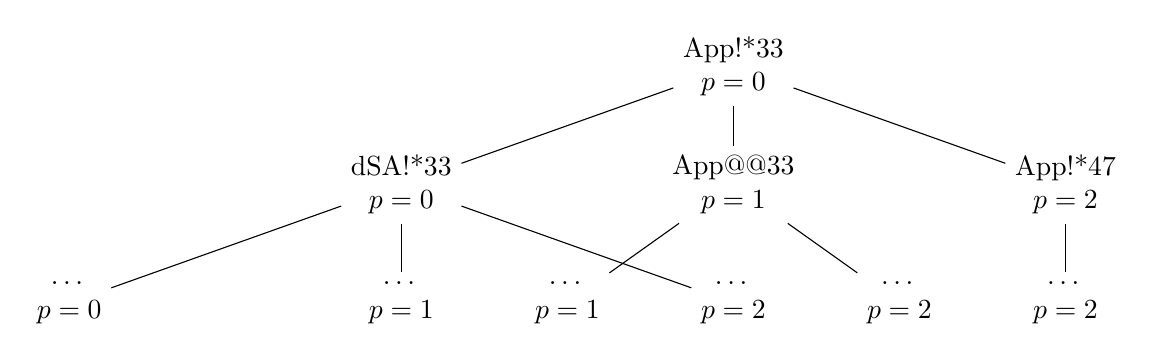
\begin{tikzpicture}[
    sibling distance=12em,
    every node/.style = {
      shape=rectangle,
      sharp corners,
      align=center
    }
  ]
    \node { App!*33 \\ $p=0$ }
      % Replace first group
      child { node { dSA!*33 \\ $p=0$ }
        child { node { \ldots \\ $p=0$ } }
        child { node { \ldots \\ $p=1$ } }
        child { node { \ldots \\ $p=2$ } }
      }
      % Replace second group
      child { node { App@@33 \\ $p=1$ }
        child { node { \ldots \\ $p=1$ } }
        child { node { \ldots \\ $p=2$ } }
      }
      % Replace third group
      child { node { App!*47 \\ $p=2$ }
        child { node { \ldots \\ $p=2$ } }
      };
  \end{tikzpicture}
  \caption{
    Slaptažodžio \textquote{App!*33}, kurio gramatika \textquote{A3S2D2},
    transformacijų medis.
  }
  \label{plot:pcfgtransforms}
\end{figure}

\subsubsubsection{Pastebėjimai}
Algoritmas pabaigą pasiekia tada, kai gramatikos arba unikalios simbolių grupės 
pasibaigia ir/arba naujiems slaptažodžiams parinkti trūksta duomenų -- raidžių, 
skaitmenų ar specialių simbolių junginių. Parenkamų slaptažodžių bei gramatikų 
ir simbolių grupių kiekiai priklauso nuo apmokymo duomenų rinkinio dydžio -- yra 
svarbu pateikti ne didelį duomenų kiekį, bet duomenis, kuriose yra daug 
pasikartojančių reikšmių. Šios pasikartojančios reikšmės yra naudojamos 
tikimybių skaičiavimams ir turi įtaką, kokie slaptažodžiai bus parenkami 
slaptažodžių parinkimo proceso pradžioje.
Algoritmas slaptažodžius parinks tik tokius, kurių gramatikos buvo užfiksuotos 
apmokymui pateiktų slaptažodžių aibėje -- naujų gramatikų ir slaptažodžių formų 
nėra.
Kadangi \textquote{PCFG} algoritmas yra pagrįstas statistinėmis tikimybėmis, 
reikalauja daug skaičiavimų.

\section{Pagrindinė tiriamoji dalis}
\subsection{Etika}
Šis darbas buvo atliktas pagal Europos elgesio kodeksą mokslinių tyrimų etikos 
klausimais
(angl. \textquote{European Code of Conduct for Research Integrity}), paruoštą 
\textquote{European Federation of Academies of Sciences and Humanities} (ALLEA) 
organizacijos. Kadangi nutekintos duomenų bazės yra sudarytos iš galimų 
vartotojų asmeninės informacijos (pvz. vardas, pavardė, elektroninis pašto 
adresas), visa informacija buvo saugiai laikoma ir tvarkoma. Asmens duomenų 
atskleidimo galimybės buvo mažinamos įgyvendinant griežtas saugumo priemones, ir 
nutekinti slaptažodžiai nebuvo testuojami su tikromis internetinių paslaugų 
vartotojų paskyromis. Darbe atskleidžiami tik patys dažniausiai pasikartojantys 
slaptažodžiai, jų sudėtingumas ir struktūra. Slaptažodžiai, kurie galėtų būti 
naudojami vartotojų identifikacijai, nebuvo atskleisti. Vartotojų asmeninė 
informacija yra nepateikta.

\subsection{Nutekintų slaptažodžių duomenų bazių analizė} \label{sec:db-analize}
Šiame darbe naudojamos dvi nutekintų slaptažodžių duomenų bazės, atvirai 
prieinamos viešais šaltiniais -- \textquote{RockYou} ir \textquote{Linkedin}. 
Dešimt dažniausiai pasikartojančių slaptažodžių duomenų bazėje 
\textquote{RockYou} yra pateikti \ref{tab:rockyou10} lentelėje, o duomenų bazėje 
\textquote{Linkedin} -- \ref{tab:linkedin10} lentelėje. Turimą 
\textquote{RockYou} nutekintą slaptažodžių duomenų bazę sudaro iš viso 
$32603388$ įrašai, iš kurių $14283864$ ($43.81 \%$ visų įrašų) slaptažodžiai yra 
unikalūs. Turimą \textquote{Linkedin} nutakintą slaptažodžių duomenų bazę sudaro 
iš viso $8616484$ įrašai, iš kurių $4878546$ ($56.61 \%$ visų įrašų) yra 
unikalūs ir su \textquote{RockYou} įrašais sutampa $664704$ (iš viso $2.04 \%$ 
visų \textquote{RockYou} irašų).

% If unsorted and unnumbered, use command:
% $ sort DB.txt | uniq -c | sort -nr | head -n 10
\begin{table}[hb]
  \centering
  \caption{
    Duomenų rinkinio \textquote{RockYou} 10 dažniausiai pasikartojančių 
    slaptažodžių.
  }
  \begin{tabular}{|c|c|}
    \hline \textbf{Kiekis} & \textbf{Slaptažodis} \\
    \hline 290729 & 123456 \\
    \hline 79076 & 12345 \\
    \hline 76789 & 123456789 \\
    \hline 59462 & password \\
    \hline 49952 & iloveyou \\
    \hline 33291 & princess \\
    \hline 21725 & 1234567 \\
    \hline 20901 & rockyou \\
    \hline 20553 & 12345678 \\
    \hline 16648 & abc123 \\
    \hline
  \end{tabular}
  \label{tab:rockyou10}
\end{table}

\ref{tab:rockyou10} lentelėje pateikti slaptažodžiai daugiausia sudaryti iš 
bendrinių daiktavardžių, paprastų skaičių ir raidžių sekų.

\begin{table}[ht]
  \centering
  \caption{
    Duomenų rinkinio \textquote{Linkedin} 10 dažniausiai pasikartojančių 
    slaptažodžių.
  }
  \begin{tabular}{|c|c|}
    \hline \textbf{Kiekis} & \textbf{Slaptažodis} \\
    \hline 75 & password1 \\
    \hline 56 & abc123 \\
    \hline 34 & fuckyou \\
    \hline 29 & monkey1 \\
    \hline 28 & iloveyou1 \\
    \hline 24 & myspace1 \\
    \hline 24 & fuckyou1 \\
    \hline 18 & number1 \\
    \hline 18 & football1 \\
    \hline 17 & nicole1 \\
    \hline
  \end{tabular}
  \label{tab:linkedin10}
\end{table}

\ref{tab:rockyou10}, \ref{tab:linkedin10} lentelėse pateikti dažniausi vartotojų 
slaptažodžiai yra daugiausia sudaryti iš lotyniškos abėcėlės raidžių bei 
skaitmenų.

\begin{figure}[!ht]
  \begin{center}
    \begin{tikzpicture}
      \begin{axis}[
        xlabel={Ilgis},
        ylabel={Kiekis},
        x unit={simboliai},
        y unit={vnt.},
        grid=major,
        grid style={dashed,gray!30},
        width=10cm,
        height=7cm,
      ]
      \addplot
        table[x=length, y=count, col sep=comma, comment 
        chars={~}]{rockyou_length.csv};
      \end{axis}
    \end{tikzpicture}
  \end{center}
  \caption{
    Nutekintos slaptažodžių duomenų bazės \textquote{RockYou} įrašų ilgiai.
  }
  \label{plot:rockyoulength}
\end{figure}

\begin{figure}[!ht]
  \begin{center}
    \begin{tikzpicture}
      \begin{axis}[
        xlabel={Ilgis},
        ylabel={Kiekis},
        x unit={simboliai},
        y unit={vnt.},
        grid=major,
        grid style={dashed,gray!30},
        width=10cm,
        height=7cm,
      ]
      \addplot
        table[x=length, y=count, col sep=comma, comment 
        chars={~}]{myspace_length.csv};
      \end{axis}
    \end{tikzpicture}
  \end{center}
  \caption{
    Nutekintos slaptažodžių duomenų bazės \textquote{myspace} įrašų ilgiai.
  }
  \label{plot:myspacelength}
\end{figure}

Toliau atlikta nutekintų slaptažodžių duomenų bazių įrašų ilgių analizė, žr. 
\ref{plot:rockyoulength}, \ref{plot:myspacelength} pav., parodo, kad daugiausia 
vartotojų sukurtų slaptažodžių yra tarp 5-10 simbolių ilgio (slaptažodžiai, 
ilgesni nei 32 simboliai, buvo atmesti pateiktuose vizualizacijose).

\subsection{Eksperimentuose taikoma strategija} \label{sec:strategy}
Su pasirinktu automatizuoto slaptažodžių parinkimo metodu ir naudojant jo 
realizacijos moksliniame straipsnyje apibrėžtus rekomenduojamus parametrus bus 
apmokytas modelis su 80 \% duomenų nuo visos pasirinktos nutekintos slaptažodžių 
duomenų bazės įrašų aibės, likusieji 20 \% bus naudojami testavimui. Nutekintoms 
slaptažodžių duomenų bazėms, kurios minėtos ir analizuotos \ref{sec:db-analize} 
skyriuje, bus naudojamos modelių apmokymui. Siekiant įvertinti automatizuoto 
slaptažodžio parinkimo metodo efektyvumą, bus generuojami tarp $10^{4}$ ir 
$10^{10}$ slaptažodžių, kurie bus testuojami su 20 \% įrašų iš apmokymui 
naudojamos duomenų bazės testavimo duomenų aibės, ir su kita, anksčiau modelio 
nematyta nutekinta slaptažodžių duomenų baze. Generuojant mažiau, nei $10^{4}$ 
slaptažodžių, \textquote{PassGAN} metodas nesugeneravo slaptžodžių, o 
\textquote{PCFG} -- turėjo mažesnį, nei 1 \% tikslumą, dėl to nebus lyginami 
mažesni, nei $10^{4}$, slaptažodžių sąrašai. Modelio apmokymas vyks su 
\textquote{RockYou} nutekinta slaptažodžių duomenų baze dėl joje esančių didelių 
slaptažodžių kiekių, palyginus su \textquote{myspace} nutekinta slaptažodžių 
duomenų baze.

Testavimas bus atliktas palyginant sugeneruotą slaptažodžių sąrašą su testavimo 
duomenų aibe \textquote{Linux} pagrindo operacinės sistemos programų paketo 
\textquote{Coreutils - GNU core utilities} įrankių \textquote{sort}, 
\textquote{comm}, \textquote{split}, \textquote{wc} pagalba \cite{Coreutils}. 
Sugeneruotas slaptažodžių sąrašas bus išrykiuotas, tarp sugeneruotos ir 
testavimo duomenų aibių bus išskirti bendri įrašai, suskaičiuotas įrašų skaičius 
ir paskaičiuota, kokią dalį sudaro bendrų įrašų skaičius testavimo duomenų 
aibės.

Slaptažodžių, sutampančių su 20 \% testavimo duomenų aibės slaptažodžiais ir su 
kitoje nutekintoje duomenų bazėje esančiais slaptažodžiais, kiekis bus 
fiksuojamas kiekvienam sugeneruotų slaptažodžių rinkiniui.

\subsection{\textquote{PassGAN} eksperimentų serija}
Šioje dalyje atliekami eksperimentai su \textquote{PassGAN} metodo realizacija 
\cite{PassGAN:impl}, generuojant slaptažodžių sąrašus pagal \ref{sec:strategy} 
skyriuje aprašyta strategija. Apmokytas modelis su 80 \% \textquote{RockYou} 
duomenų rinkiniu, ir, testuojant su 20 \% to paties duomenų rinkinio testavimo 
duomenų aibe, rezultatai pateikti \ref{tab:passganrockyouresults} lent., kurioje 
matyti panašūs rezultatai į \textquote{PassGAN} metodo mokslinio straipsnio 
autoriaus rezultatus, pateiktus \ref{tab:passganoriginalresults} lent.

\begin{table}[hb]
  \centering
  \caption{
    Slaptažodžių, sugeneruotų \textquote{PassGAN} metodu, apmokytų 80 \% 
    \textquote{RockYou} duomenų ir sutampančių su \textquote{RockYou} testavimo 
    duomenų aibe.
  }
  \begin{tabular}{|c|c|c|}
    \hline \textbf{Slaptažodžių kiekis} & \textbf{Unikalūs slaptažodžiai} & 
    \textbf{Sutampančių slaptažodžių kiekis} \\
    \hline $10^4$ & 9040 & $0.028584$ \% \\
    \hline $10^5$ & 95295 & $0.254988$ \% \\
    \hline $10^6$ & 885174 & $1.505298$\% \\
    \hline $10^7$ & 7489667 & $5.285309$ \% \\
    \hline $10^8$ & 57162878 & $12.358798$ \% \\
    \hline $10^9$ & 390305149 & $21.805633$ \% \\
    \hline $10^{10}$ & 2379342789 & $32.126489$ \% \\
    \hline
  \end{tabular}
  \label{tab:passganrockyouresults}
\end{table}

Atlikus analizę \textquote{PassGAN} metodu sugeneruotų slaptažodžių dublikatų 
kiekio, rezultatai pateikti \ref{plot:passganrockyouresults} pav., kuriose taip 
pat matyti panašūs dublikuotų slaptažodžių kiekiai, kaip pateikta 
\ref{plot:passganoriginalresults} pav.

\begin{figure}[!ht]
  \begin{center}
    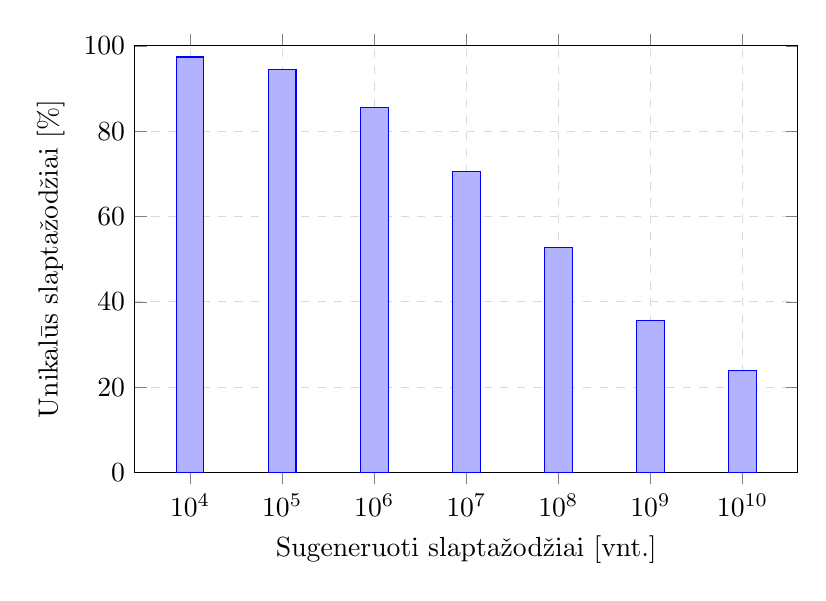
\begin{tikzpicture}
      \begin{axis}[
        ybar,
        xlabel={Sugeneruoti slaptažodžiai},
        ylabel={Unikalūs slaptažodžiai},
        x unit={vnt.},
        y unit={\%},
        ymin=0,
        ymax=100,
        xticklabels={,,$10^4$,$10^5$,$10^6$,$10^7$,$10^8$,$10^9$,$10^{10}$},
        grid=major,
        grid style={dashed,gray!30},
        width=10cm,
        height=7cm,
      ]
      \addplot coordinates {
        (1, 97.38)
        (2, 94.4)
        (3, 85.5972)
        (4, 70.64483)
        (5, 52.815412)
        (6, 35.621683)
        (7, 23.793428)
      };
      \end{axis}
    \end{tikzpicture}
  \end{center}
  \caption{
    Unikalių slaptažodžių, sugeneruotų \textquote{PassGAN} metodu, kiekis.
  }
  \label{plot:passganrockyouresults}
\end{figure}

Palyginus \ref{tab:passganrockyouresults} lent. ir 
\ref{plot:passganrockyouresults} pav. pateiktus rezultatus, kurie yra panašūs į 
\textquote{PassGAN} mokslinio straipsnio rezultatus, atliktas palyginimas su 
\textquote{PassGAN} mokslinio straipsnio autoriaus gautais rezultatais su tą 
pačia nutekinta slaptažodžių duomenų baze -- \textquote{RockYou} (80 \% 
slaptažodžių modelio apmokymui, likusieji 20 \% testavimui) -- kurio rezultatai 
pateikti \ref{plot:passgancomparison} pav.

\begin{figure}[!ht]
  \begin{center}
    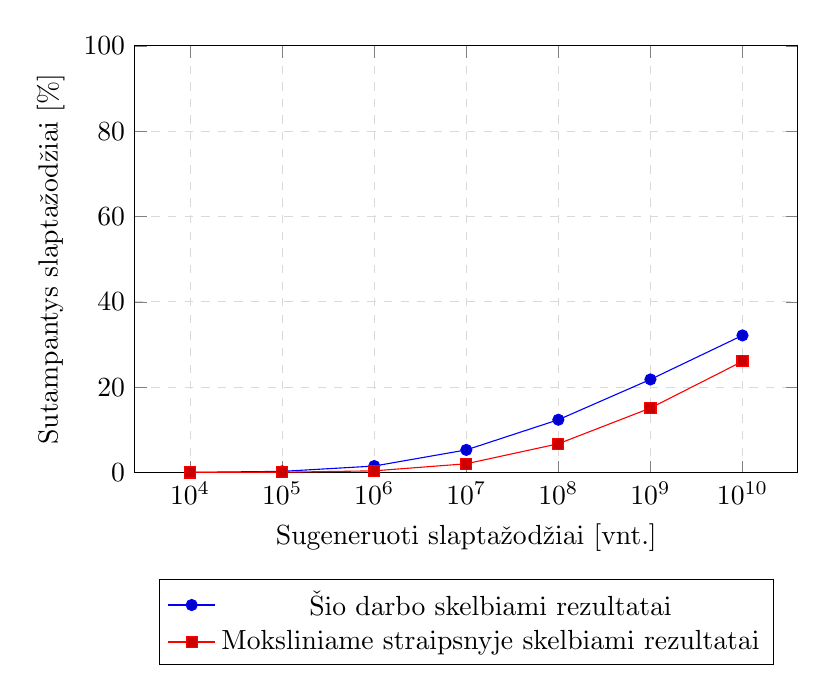
\begin{tikzpicture}
      \begin{axis}[
        xlabel={Sugeneruoti slaptažodžiai},
        ylabel={Sutampantys slaptažodžiai},
        x unit={vnt.},
        y unit={\%},
        ymin=0,
        ymax=100,
        xticklabels={,,$10^4$,$10^5$,$10^6$,$10^7$,$10^8$,$10^9$,$10^{10}$},
        grid=major,
        grid style={dashed,gray!30},
        width=10cm,
        height=7cm,
        legend style={at={(0.5,-0.25)}, anchor=north}
      ]
      \addplot coordinates {
        (1, 0.028584)
        (2, 0.254988)
        (3, 1.505298)
        (4, 5.285309)
        (5, 12.358798)
        (6, 21.805633)
        (7, 32.126489)
      };
      \addplot coordinates {
        (1, 0.005)
        (2, 0.048)
        (3, 0.381)
        (4, 2.038)
        (5, 6.726)
        (6, 15.094)
        (7, 26.036)
      };
      \legend{
        Šio darbo skelbiami rezultatai,
        Moksliniame straipsnyje skelbiami rezultatai
      }
      \end{axis}
    \end{tikzpicture}
  \end{center}
  \caption{
    Sutampančių su 20 \% \textquote{RockYou} duomenų rinkinio testavimo aibe 
    slaptažodžių dalis, palyginus su \textquote{PassGAN} mokslinio straipsnio 
    autoriaus rezultatais.
  }
  \label{plot:passgancomparison}
\end{figure}

Įvertinus \ref{plot:passgancomparison} pav. pateiktą informaciją, nustatyta, kad 
iki $10^7$ sugeneruotų slaptažodžių, slaptažodžių kiekis, sutampantis su 
testavimo duomenų aibe, sutampa (tarp 1-2 \%), o didesniems generuojamų 
slaptažodžių kiekiams -- šiame darbe apmokytu modeliu maždaug 4-6 \% daugiau 
slaptažodžių parenka. Toks slaptažodžių parinkimo tikslumo pakilimas yra 
priskiriamas nutekintos slaptažodžių duomenų bazės \textquote{RockYou} 
išmaišymui prieš padalinant į apmokymo ir testavimo aibes. Slaptažodžiai, su 
kuriais buvo testuojamas modelis aukščiau minėtame straipsnyje, galimai pateko į 
apmokymo duomenų aibę šiame darbe, todėl parinkimo tikslumas neryškiai skiriasi.

Toliau, patikrinus sugeneruotus $10^4$-$10^{10}$ slaptažodžių sąrašus su 
\textquote{Linkedin} testavimo duomenų rinkiniu, buvo atlikta analogiška 
rezultatų analizė, kaip aukščiau, ir analizės rezultatai pateikti -- sutampančių 
slaptažodžių kiekis procentais \ref{tab:passganlinkedinresults} lent.

\begin{table}[hb]
  \centering
  \caption{
    Slaptažodžių, sugeneruotų \textquote{PassGAN} metodu, apmokytų 80 \% 
    \textquote{RockYou} duomenų ir sutampančių su \textquote{Linkedin} testavimo 
    duomenų aibe.
  }
  \begin{tabular}{|c|c|c|}
    \hline \textbf{Slaptažodžių kiekis} & \textbf{Unikalūs slaptažodžiai} & 
    \textbf{Sutampančių slaptažodžių kiekis} \\
    \hline $10^4$ & 9040 & $0.011684$ \% \\
    \hline $10^5$ & 95295 & $0.103781$ \% \\
    \hline $10^6$ & 885174 & $0.608665$ \% \\
    \hline $10^7$ & 7489667 & $2.233555$ \% \\
    \hline $10^8$ & 57162878 & $5.586419$ \% \\
    \hline $10^9$ & 390305149 & $10.574647$ \% \\
    \hline $10^{10}$ & 2379342789 & $16.681897$ \% \\
    \hline
  \end{tabular}
  \label{tab:passganlinkedinresults}
\end{table}

\begin{figure}[!ht]
  \begin{center}
    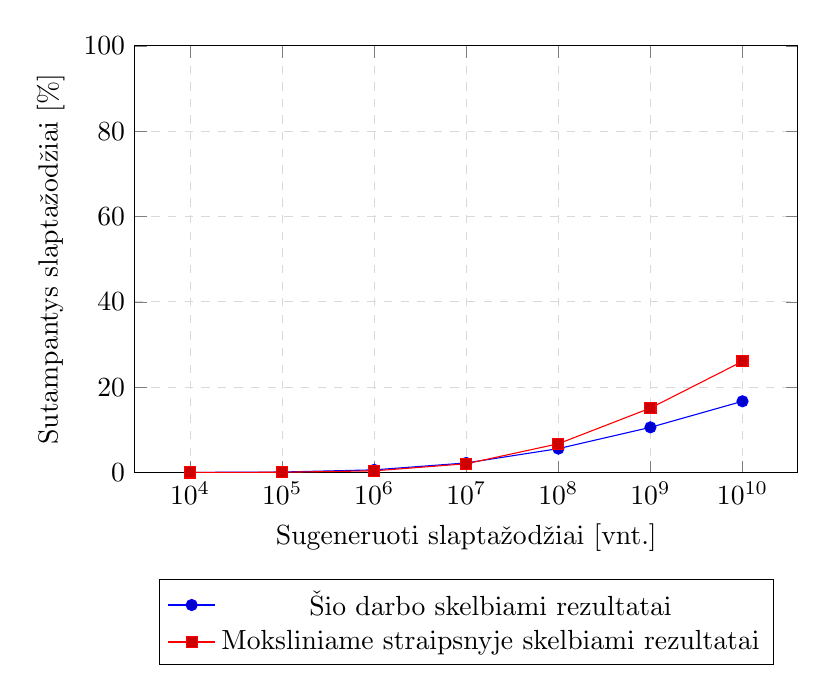
\begin{tikzpicture}
      \begin{axis}[
        xlabel={Sugeneruoti slaptažodžiai},
        ylabel={Sutampantys slaptažodžiai},
        x unit={vnt.},
        y unit={\%},
        ymin=0,
        ymax=100,
        xticklabels={,,$10^4$,$10^5$,$10^6$,$10^7$,$10^8$,$10^9$,$10^{10}$},
        grid=major,
        grid style={dashed,gray!30},
        width=10cm,
        height=7cm,
        legend style={at={(0.5,-0.25)}, anchor=north}
      ]
      \addplot coordinates {
        (1, 0.011684)
        (2, 0.103781)
        (3, 0.608665)
        (4, 2.233555)
        (5, 5.586419)
        (6, 10.574647)
        (7, 16.681897)
      };
      % SITUS REIKIA PAKEISTI
      \addplot coordinates {
        (1, 0.005)
        (2, 0.048)
        (3, 0.381)
        (4, 2.038)
        (5, 6.726)
        (6, 15.094)
        (7, 26.036)
      };
      \legend{
        Šio darbo skelbiami rezultatai,
        Moksliniame straipsnyje skelbiami rezultatai
      }
      \end{axis}
    \end{tikzpicture}
  \end{center}
  \caption{
    Sutampančių su 20 \% \textquote{RockYou} duomenų rinkinio testavimo aibe 
    slaptažodžių dalis, palyginus su \textquote{PassGAN} mokslinio straipsnio 
    autoriaus rezultatais.
  }
  \label{plot:passgancomparison}
\end{figure}
\subsection{\textquote{PCFG} eksperimentų serija}
Šioje dalyje atliekami eksperimentai su \textquote{PCFG} metodo realizacija 
\cite{PCFG:impl}, generuojant slaptažodžių sąrašus pagal \ref{sec:strategy} 
skyriuje aprašyta strategija.

\begin{figure}[!ht]
  \begin{center}
    \begin{tikzpicture}
      \begin{axis}[
        xlabel={Sugeneruoti slaptažodžiai},
        ylabel={Sutampantys slaptažodžiai},
        ymax=100,
        x unit={vnt.},
        y unit={\%},
        grid=major,
        grid style={dashed,gray!30},
        width=10cm,
        height=7cm,
        % legend style={at={(0.5,-0.5)}, anchor=north}
      ]
      \addplot[color=red, mark=*]
        table[x=power of 10, y=matches, col sep=comma]{pcfg_ROCKYOU_80.csv};
      % \addplot[color=blue, mark=*]
      %   table[x=column 1, y=column 2, col sep=comma]{table2.csv};
      % \legend{Case 1,Case 2}
      \end{axis}
    \end{tikzpicture}
  \end{center}
  \caption{
    Sugeneruotų slaptažodžių, sutampančių su 20 \% testavimo duomenų rinkinyje 
    esančiais slaptažodžiais, dalis.
  }
  \label{plot:kazkoks}
\end{figure}

\sectionnonum{Išvados}
Išvadose ir pasiūlymuose, nekartojant atskirų dalių apibendrinimų,
suformuluojamos svarbiausios darbo išvados, rekomendacijos bei pasiūlymai.
% Ar atlikta studija sėkmingai išsprendė užsibrėžtą tikslą?
% Kokie apribojimai buvo taikomi, kurie trukdė atlikti tyrimą?
% Ar gauti rezultatai yra patikimi?
% Ar buvo atliktas palyginimas su kitų autorių analogiškais rezultatais?
% Kaip rezultatai gali būti panaudoti ateityje?
% Kokio tipo naują informaciją/sprendimą/tyrimą galima pažymėti?
% Kokias naujas idėjas ir pasiūlymus iškelia gauti rezultatai?

\sectionnonum{Conclusions}
Šiame skyriuje pateikiamos išvados (reziume) anglų kalba.

\printbibliography[heading=bibintoc]

\appendix  % Priedai
% Prieduose gali būti pateikiama pagalbinė, ypač darbo autoriaus savarankiškai
% parengta, medžiaga. Savarankiški priedai gali būti pateikiami kompiuterio
% diskelyje ar kompaktiniame diske. Priedai taip pat vadinami ir numeruojami.
% Tekstas su priedais siejamas nuorodomis (pvz.: \ref{img:mlp}).

% \section{Niauroninio tinklo struktūra}
% \begin{figure}[H]
%     \centering
%     \includegraphics[scale=0.5]{img/MLP}
%     \caption{Paveikslėlio pavyzdys}
%     \label{img:mlp}
% \end{figure}

\section{Eksperimentinio palyginimo rezultatai}

\end{document}
